\documentclass[../main/thesis.tex]{subfiles}
\begin{document}
\newpage
%% Theory

\chapter{Radiation and Radiotherapy}
\label{theory}
\section{Radiation}
\label{t-radiation}
\textit{Radiation} is defined as the emission and propagation of energy through space or a material medium. Previously radiation was split into groups depending on if it was transferred through particles or waves. This was changed after 1924 when Louis de Broglie claimed that all matter has a wave-like nature. Now, \textit{particle radiation} refers to energy propagated by particles with a definite rest mass and within limits at any instant have a definite momentum and defined position. A particle beam is a group of particles that move in the same direction, similar to a light beam. Examples of these particles are electrons, neutrons, protons, and heavy ions. \textit{Electromagnetic radiation} is energy propagated  by the massless photons in phenomena such as light waves, radio waves, microwaves, X-rays, and gamma ($\gamma$) rays. Electromagnetic waves propagate at the speed of light and are represented by the spatial intensity variations of an electric field and a magnetic field. \citep[chap. 1]{Khan} 

\textit{Ionizing radiation} carries enough energy to break molecular bonds by \textit{ionizing} atoms it passes, meaning that the atom acquires a positive or negative charge. If the radiation strips an electron from the atom, it becomes a positive ion. If a stripped electron later combines with a neutral atom, it becomes a positive ion. Charged particles with enough kinetic energy is called \textit{directly ionizing radiation} because they can ionize atoms through collisions. Uncharged particles are known as \textit{indirectly ionizing radiation} as they \textit{excite} atoms, raising electrons to higher energy levels. An excited atom can later emit directly ionizing radiation through an electron. \citep[chap. 5]{Khan} See section \ref{t-int} for more on this.

%Mention MIP!

%Radioactivity?

%Sources of radiation?

\subsection{Interactions of Radiation with Matter}
\label{t-int}
\subsubsection{Interactions of charged particles with matter}
\label{t-cp}
Charged particles, for example protons, primarily react by ionization and excitation. Electrons also commonly react through bremsstrahlung (deceleration radiation), where the particle is decelerated and emits the lost kinetic energy as a photon. When charged particles travel through a medium, they interact with atomic electrons and nuclei through the Coulomb force. These interactions can be inelastic collisions with atomic electrons, or elastic scattering without energy loss. In the inelastic collisions, the particle looses part of its kinetic energy to produce ionizations and excitations of atoms. This results in energy being absorbed in the medium as the particle is decelerated. \citep[chap. 5 $\&$ 27]{Khan} 

\textit{Stopping power} is the average rate of energy loss of a particle per unit path length ($-dE/dx$) in a medium. The \gls{let} of a particle is the energy locally deposited per length and is usually expressed in $MeV/cm$ or $keV/{\mu}m$. The \gls{let} will always be equal to or smaller than the stopping power. These parameters are used to describe energy deposition in matter and the biological effect of radiation (see section~\ref{t-bio}). The \gls{let} of a heavy charged particle (a particle of equal or greater mass than a proton) travelling through matter is inversely proportional to the square of its velocity. This means that as the particle looses energy and slows down, the rate of energy loss will increase and the particle slows down at a faster rate. The rate of energy loss (and energy deposition in the medium) becomes maximum as the particle velocity approaches zero. This leads to the particle stopping relatively quickly after travelling a certain distance and makes it possible to define a range for a certain type of particle with a defined energy in a type of matter. The intensity of a particle beam plotted versus depth in tissue can be seen in figure~\ref{fig-range} where the sudden drop in the proton plots is defined as the particle's range for that energy. \citep[chap. 27]{Khan}

\begin{figure}[h]
	\centering
	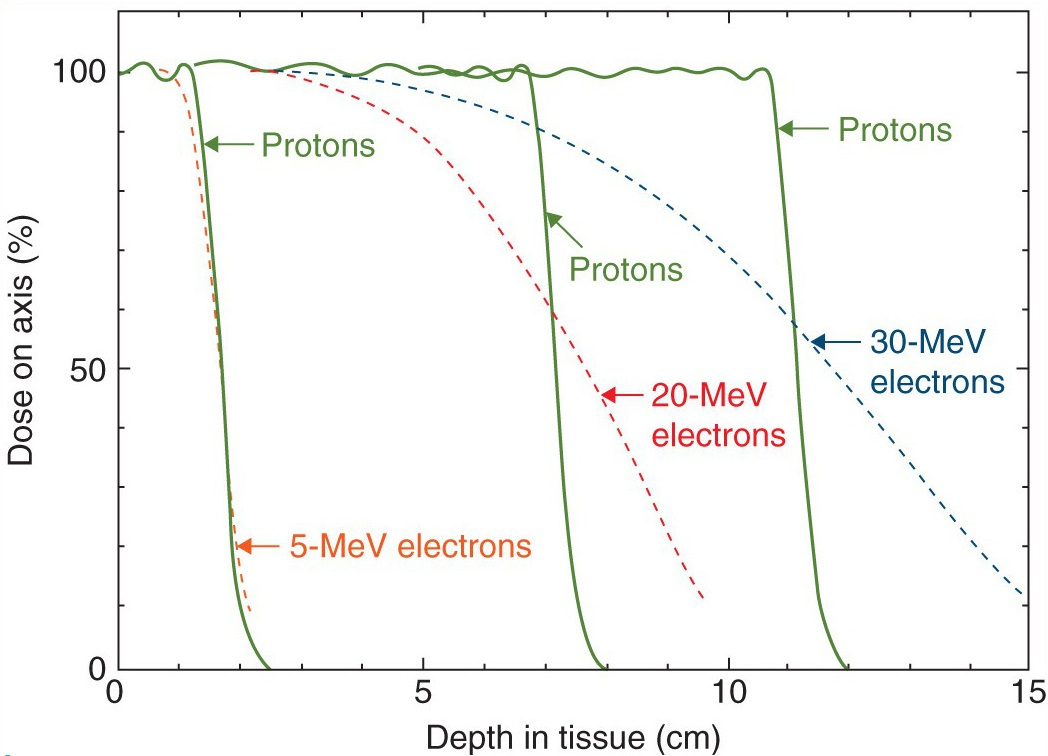
\includegraphics[width=0.8\textwidth]{figure_5_15.jpg}
	\caption{Comparison of depth dose distribution for protons and electrons of different energies. \citep[fig. 5.15]{Khan}}
	\label{fig-range}
\end{figure}

\subsubsection{Interactions of photons with matter}
\label{t-photon}
The five dominating processes for photon interactions with matter are Rayleigh scattering, the photoelectric effect, the Compton effect, pair production, and photodisintegration. Rayleigh scattering happens when a low energy photon collides with an electron and is scattered to a different angle. This does not deposit any energy in the medium, but the photon is scattered away from its original path. The photoelectric effect is a phenomenon where all the energy of a photon is absorbed in an atom. This leads to one of the orbital electrons being emitted, and the shell vacancy will lead to emission of X-rays as a higher energy electron fills the vacancy. Occasionally, these X-rays will also cause more electrons to be emitted. The Compton effect is when a photon collides with an atomic bound electron, scattering the photon and transferring some of its energy to the electron. This is given to the electron as kinetic energy. Pair production can happen with photons of energy greater than 1.022~MeV, where a photon travelling near an atomic nucleus gives all its energy to produce an electron and a positron. The positron will later find an atomic electron and they will annihilate each other by producing two photons of 0.511~MeV each. A high energy photon can cause photodisintegration by reacting with an atomic nucleus, leading to a nuclear reaction. \citep[chap. 2 $\&$ 5]{Khan} 

Due to all the above processes, a photon travelling through matter will at each instant in time have a certain chance of being absorbed or scattered by the medium. Because of this, the intensity of a photon beam will start to go down instantly when it leaves vacuum, but will take a very long time to be reduced to zero, see figure~\ref{fig-photon}. It is therefore very difficult to simply define the range of a photon beam, as can be done with a beam of heavy charged particles. The reduction in the number of photons is proportional to the number of incident photons through the \textit{attenuation coefficient}. \citep[chap. 5]{Khan} 

\begin{figure}[h]
	\centering
	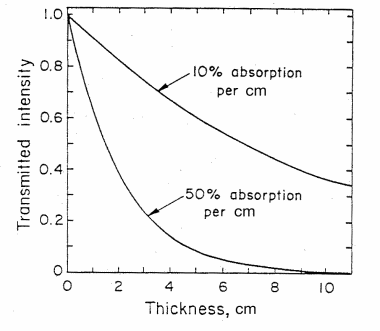
\includegraphics[width=0.6\textwidth]{asu-photon.png}%4.1?
	\caption{Photon intensity through an absorber as a function of thickness \citep{asu2000}}
	\label{fig-photon}
\end{figure}

\subsection{Biological Effects of Radiation}
\label{t-bio}
As discussed in the previous sections, radiation travelling through matter deposits energy in the medium. Examining the effects of this in biological tissue is an extremely complex field. Non-ionizing radiation can heat the matter it passes through. Ionizing radiation is much more dangerous as it breaks molecular bonds, causing molecules to fall apart. This can cause massive damage to tissue cells, change the genetic material (DNA), and destroy the components that produce red blood cells. \citep[chap. 43]{UniversityPhysics} 

When a cell has been damaged by radiation, there are three possible effects: The cell dies, the cell is repaired correctly, or the cell is repaired incorrectly. The human body has very effective repair mechanisms which constantly repair cellular damage, including damage to DNA. Occasionally, these repair mechanisms will perform their function incorrectly, which can result in cells that cannot perform their normal function, or cells that damage other cells. Some of these cells are unable to reproduce themselves, while others reproduced at an uncontrolled rate, which can be the cause of cancers.\citetext{\citeauthor{jlab}}

To be able to describe the quantity of ionizing radiation for all energies, materials, and types of radiation, it is common to use the quantity \textit{absorbed dose}, or simply \textit{dose}, which can be used as a measure of the biologically significant effects that ionizing radiation produces. It is defined as the radiation energy delivered to tissue per unit mass. The SI unit for dose is gray (Gy), where $1 Gy = 1 J/kg$. The quantity \textit{dose equivalent} has been defined because the biological effects of radiation depend on the type of radiation in addition to the dose. Dose equivalent is the dose multiplied by a quality factor for the type of radiation, in units of sievert (Sv). $1 Sv = 1 J/kg$. Additionally, the sensitivity to radiation-induced effects will vary for different types of tissue, leading to the definition of \textit{effective dose equivalent}, defined as "the sum of the weighted dose equivalents for irradiated tissues or organs". \citep[chap. 8 $\&$ 16]{Khan} 

%Dosimetry, microdosimetry?

%Vann vs tissue?
%Rekkevidde i vann?

\section{Radiation Therapy}
\label{t-therapy}
Radiation therapy, also known as radiotherapy, is therapy using the biological effects of ionizing radiation to kill or control cancer cells. One of the main principles behind radiotherapy's effectiveness in treating cancer is that radiation causes much more damage to rapidly dividing cells, and tumor cells divide extremely rapidly \citep[chap. 45]{Serway}. Roughly half of all cancer patients receive radiotherapy as a part of their treatment. The radiation can originate from a machine outside the body (external beam radiation therapy), or from a radioactive source being placed into the body (internal radiation therapy). Traditional external beam radiation therapy is delivered using photon beams (photon therapy), but treatment with beams of heavy charged particles (particle therapy), like protons (proton therapy) or carbon ions, are becoming more common. Electron beam therapy is also used, mainly to treat cancer close to the surface of the body. \citep{nih}

The radiation will also damage healthy tissue, but a lot of work is put into reducing this as much as possible. Planning and simulations are done to increase the certainty of avoiding complications. Detailed imaging scans are done to get a 3D map of the patient's tumor and surrounding areas. The basis for these maps are usually \gls{CT} scans, but can also be combined with \gls{MRI}, \gls{PET}, X-ray images, or ultrasound scans \citep{nih}. One of the main reasons for \gls{CT}'s importance for photon therapy is that as it is based on photon beams, a \gls{CT} scan also yields the body's tissue-density information and photon attenuation coefficient, which is needed for photon therapy planning.  \citep[chap. 12]{Khan}

The particle beams of external beam radiation therapy are of high energy and needs to be produced in or near the treatment machine. For photon therapy, it is most common to accelerate photons using a \gls{linac}, which is small enough to fit inside the same room as the patient table \citep{nih}. For particle therapy a bigger and more expensive accelerator is needed to accelerate the particles to high enough energies. For proton therapy a cyclotron or a synchrotron is used. \citep[chap. 27]{Khan}

A patient treatment dose is usually delivered once per day every workday for 4-6 weeks. One delivery is called a fraction. Fractionation is done for multiple reasons: One is to allow healthy tissue time to repair the damage from radiation. Another is to increase the chance of hitting the cancer cells at a time when they are vulnerable. Fractionation also helps to minimize the effects of random variations in the patient's position and internal geometry. \citep{fractionation} \citep{hysing-uncertain}

As already mentioned, radiation therapy also damages healthy tissue, which can produce both acute (early) and chronic (late) side effects. Acute side effects occur before the treatment ends, and is usually temporary. Examples include skin irritation, hair loss, fatigue and nausea. Chronic side effects develop months to decades after treatment is complete. Examples are skin damage, memory loss, infertility and secondary cancer. Secondary cancer is the development of a new cancer in a person that has previously had cancer. As this takes a long time to develop, it might not be a very large problem for older patients, but it is critical to avoid secondary cancer when treating cancer in children and adolescents. \citep{nih} 

When plotting the absorbed dose in water (or tissue), the differences between photon beams and heavy charged particle beams become even more apparent than when plotting the intensities (section \ref{t-int}). Figure \ref{fig-photonproton} shows the relative dose deposited in water for a proton and a photon beam. The photon beam's maximum is very close to the surface, and the photons will damage tissue far into the body. Also, if the tumor is deep into the body, and the beam only comes from one direction, the photons will have to do a lot of damage to the skin to be able to do enough damage to the tumor. Protons (and other heavy charged particles) on the other hand have their maximum deeper into the material, in what is called the \textit{Bragg peak}. Protons deposit less energy before the maximum, and close to no damage behind the maximum. 

\begin{figure}[h]
	\centering
%	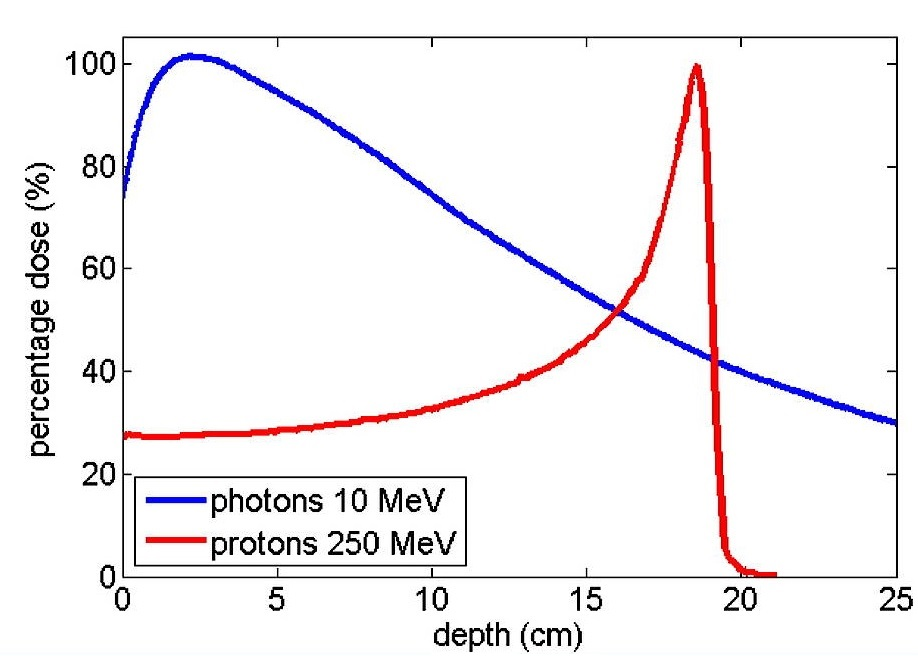
\includegraphics[width=0.7\textwidth]{swiss-photonproton.jpg}
%	\caption{Percentage depth dose for a photon beam and a proton beam in water. \citep{swiss}}
	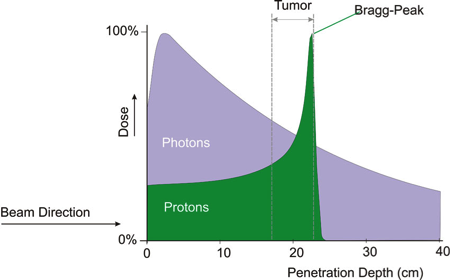
\includegraphics[width=0.7\textwidth]{pcure-photonproton.png}
	\caption{Percentage depth dose for a photon beam and a proton beam in tissue. \citetext{\citeauthor{pcure}}}
	\label{fig-photonproton}
\end{figure}

%4.18, 9.3, 27.1

\subsection{Proton Therapy} %Burde bytte til particle therapy, eller legge til lite Carbon Therapy section
\label{t-proton}
Proton therapy is radiation therapy using high energy proton beams. The main principle behind the use of proton therapy is to exploit the Bragg peak to deposit a high dose to a tumor, with low dose delivered in front of it, and close to no dose behind. The Bragg peak is very narrow and is not able to cover most tumors, which has lead to the use of superposition of multiple beams of different energies. This superposition is called a \gls{SOBP}, see figure \ref{fig-sobp}. A \gls{SOBP} has a lot higher dose deposited in front of the tumor than a single proton beam, but it is still lower than that of a photon beam. The dose behind the tumor is still low. \citep[chap. 27]{Khan}

\begin{figure}[h!]
	\centering
	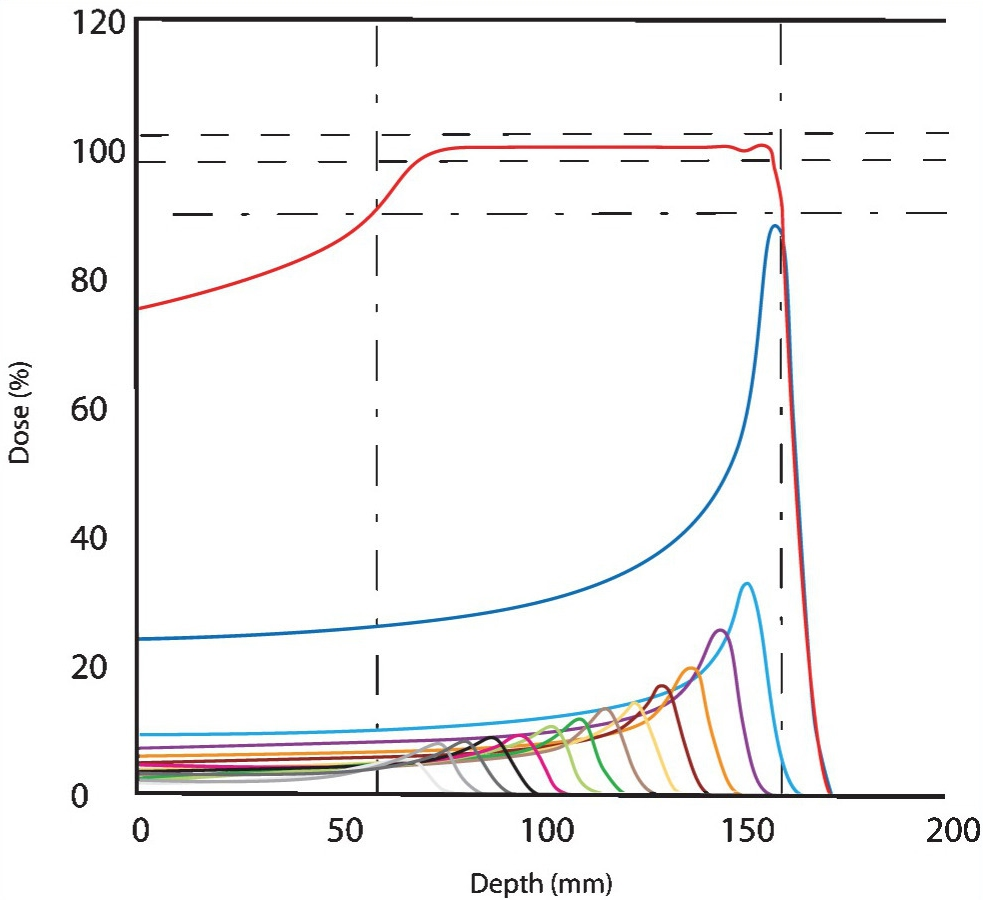
\includegraphics[width=0.5\textwidth]{figure_27_10.jpg}
	\caption{\gls{SOBP} depth dose distribution \citep[fig. 27.10]{Khan}}
	\label{fig-sobp}
\end{figure}

%Bilde av range endring? phys251 pdf

The shape of the \gls{SOBP} makes it possible to treat tumors with a lot less dose to the surrounding tissue than with photon therapy, which has two main benefits. One is the ability to treat tumors in close proximity to critical organs without damaging said organ. The other is to avoid the chronic side effects mentioned in section \ref{t-therapy}, which is very important when treating children with cancer \citep[chap. 27]{Khan}. Figure \ref{fig-photonproton-dose} compares photon (A) and proton (B) beams, where red is high dose, blue is low dose, and gray is negligible dose. 

\begin{figure}[h]
	\centering
	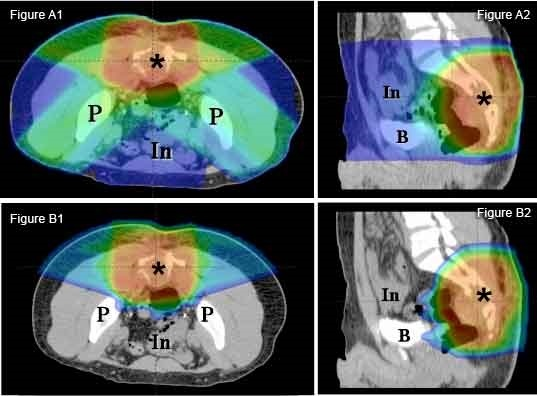
\includegraphics[width=0.8\textwidth]{pcure-dose-distribution.jpeg}
	\caption{Photon (A1 \& A2) and proton (B1 \& B2) beam dose distributions. \citetext{\citeauthor{pcure}}}
	\label{fig-photonproton-dose}
\end{figure}

The geometrical accuracy in proton therapy is a lot more critical than in photon therapy. While a geometrical error between planning and delivery in photon therapy will give a smaller under-dosage to the tumor and over-dosage to surrounding tissue, similar errors in proton therapy could cause part of the tumor receiving no dose at all and healthy tissue receiving full dose, see figure \ref{fig-miss}. Geometrical uncertainties can come from setup and anatomical variations, biological considerations, organ motion, and dose calculation approximations. \citep{Paganetti-range} 

As mentioned in section \ref{t-therapy}, photon \gls{CT} yields the patient's photon attenuation coefficient that is needed for photon therapy, but for proton therapy the stopping power is needed to greatly reduce range errors. Therefore proton \gls{CT} imaging techniques are being developed, based on the same principles as conventional \gls{CT}, but using low-intensity proton beams instead of photon beams. \citep{proton-ct}

Proton therapy can theoretically be delivered in fewer fractions than photon therapy due to lower dose to surrounding tissue, but this is more risky in case the target is missed.

\begin{figure}[h]
	\centering
	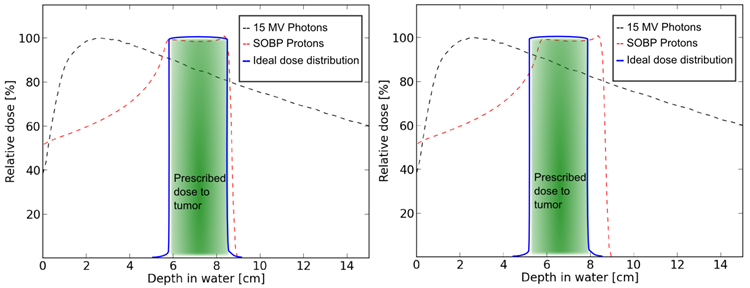
\includegraphics[width=\textwidth]{ksyh-miss.png}
	\caption{Comparison of dose distribution with correct (left) and incorrect (right) range assumptions. \citep{ksyh-phys251}}
	\label{fig-miss}
\end{figure}

%%XXX RBE and 1.1 thingy? Mention in 3DMiMic introduction

%%XXXX: Need to add something about Carbon therapy
%Make this more general "particle therapy", then add a paragraph about carbons.
\newpage
\subsection{Carbon Therapy}
\label{t-carbon}
%front, tail, sides, accelerator, rbe?
Carbons have also been used clinically for radiotherapy since 1994 in Japan, and 2002 in Germany. Data from these centers suggest that carbon therapy is superior to proton therapy for certain types of cancer. By comparing depth dose distributions, figure \ref{fig-carbon}, the carbon ion shows a sharper Bragg peak, but the dose is not reduced to zero after the Bragg peak. This suggests that carbon therapy might be worse than proton therapy when there is a critical organ just behind the tumor. For certain cancer types can however benefit from the sharper Bragg peak, lower entrance dose, and lower lateral spread of dose \ref{fig-carbon}. As carbons are heavier, they also require more complex and expensive accelerators than protons. \citep{ksyh-phys251}

\begin{figure}[h]
	\centering
	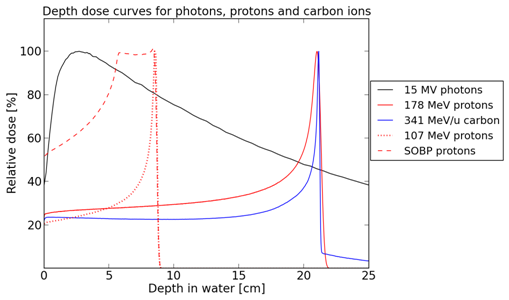
\includegraphics[width=0.7\textwidth]{carbon.png}
	\caption{Comparison of photon, proton, and carbon depth dose distributions. \citep{ksyh-phys251}}
	\label{fig-carbon}
\end{figure}

\end{document}